\documentclass{article}
\usepackage{graphicx}
\usepackage{tikz}
\usepackage{pgfplots}

\title{Statistics Notes}
\author{Your Name}

\begin{document}
\maketitle

\section{Introduction}
Statistics is the study of data collection, analysis, interpretation, presentation, and organization. It involves various concepts such as sets, probability, groups, etc.

\section{Sets}
A set is a collection of distinct elements. It can be represented using set notation, such as $A = \{a, b, c\}$, where $a$, $b$, and $c$ are the elements of the set $A$.

\section{Probability}
Probability is a measure of the likelihood of an event occurring. It is represented as a number between 0 and 1, where 0 indicates impossibility and 1 indicates certainty.

\section{Graphs}
\begin{figure}[ht]
    \centering
    \begin{tikzpicture}
        \begin{axis}[
            xlabel={Time},
            ylabel={Value},
            xmin=0, xmax=10,
            ymin=0, ymax=100,
            xtick={0,2,4,6,8,10},
            ytick={0,20,40,60,80,100},
            legend pos=north west,
            grid style=dashed,
        ]
        \addplot[
            color=blue,
            mark=square,
        ]
        coordinates {
            (0,0)(2,20)(4,40)(6,60)(8,80)(10,100)
        };
        \legend{Data}
        \end{axis}
    \end{tikzpicture}
    \caption{Example line graph}
    \label{fig:line-graph}
\end{figure}

\section{Venn Diagrams}
\begin{figure}[ht]
    \centering
    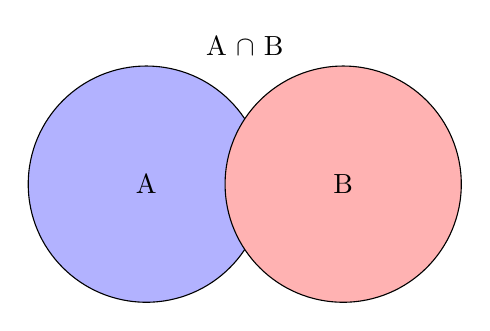
\begin{tikzpicture}
        \draw[fill=blue!30] (0,0) circle (1.5cm);
        \draw[fill=red!30] (2.5,0) circle (1.5cm);
        \node at (0,0) {A};
        \node at (2.5,0) {B};
        \node at (1.25,1.75) {A $\cap$ B};
    \end{tikzpicture}
    \caption{Example Venn diagram}
    \label{fig:venn-diagram}
\end{figure}

\section{3D Models}
\begin{figure}[ht]
    \centering
    \includegraphics[width=0.5\textwidth]{3d-model.png}
    \caption{Example 3D model}
    \label{fig:3d-model}
\end{figure}

\end{document}
